\begin{document}
\subsection{レストラン画面}
\subsubsection{食事情報閲覧画面}
図\ref{fig:restaurant}に食事情報閲覧画面を示す.
\begin{figure}[H]
 \centering
   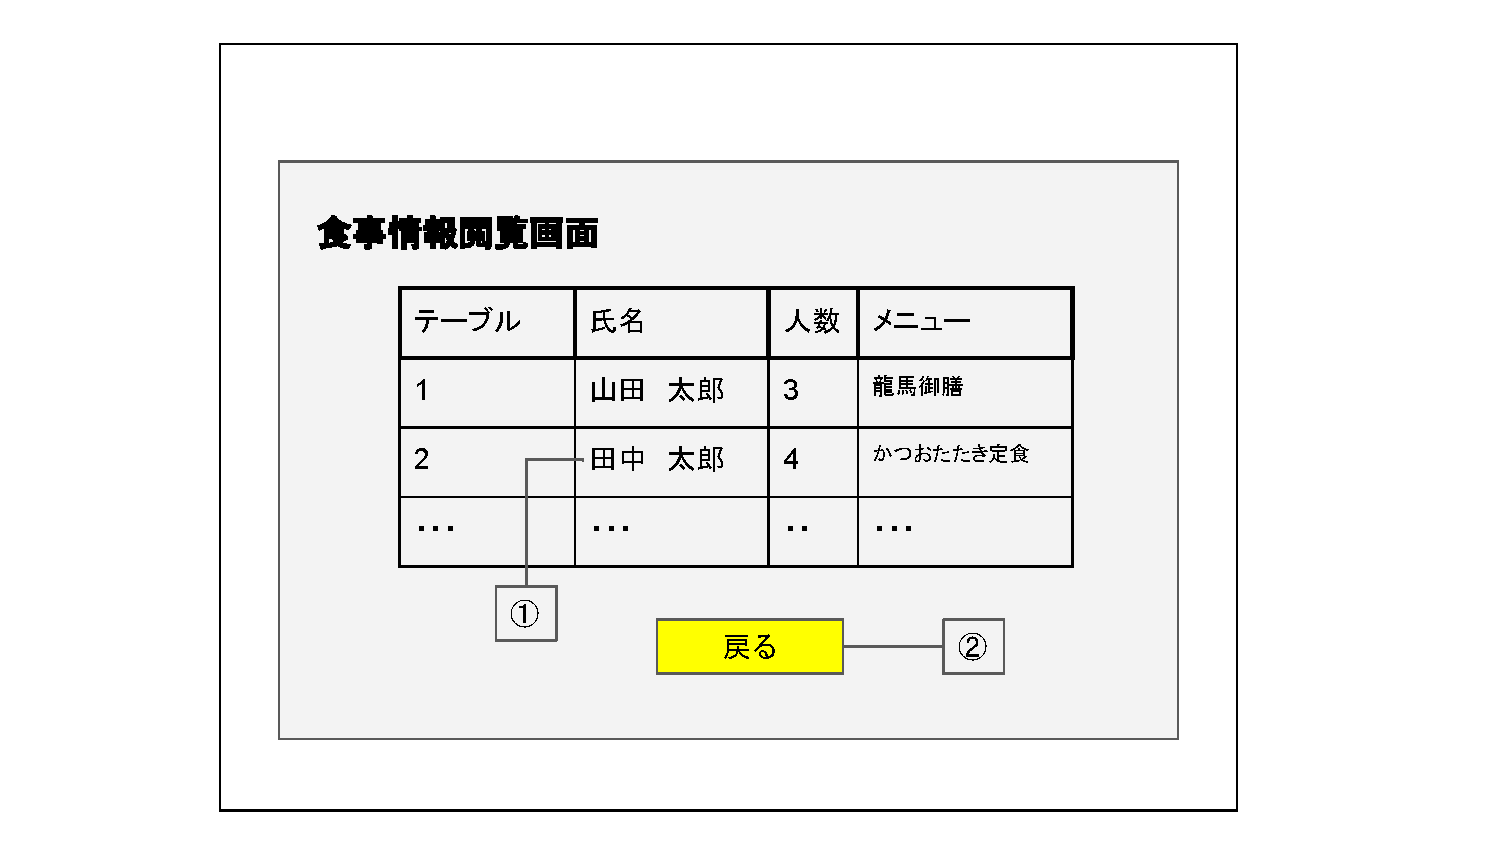
\includegraphics[width=150mm]{UI-restaurant/user-restarant00.pdf}
 \caption{食事情報閲覧画面}
 \label{fig:restaurant}
\end{figure}

\begin{enumerate}
\renewcommand{\labelenumi}{\textcircled{\scriptsize \theenumi}}
\item お客様情報詳細 \\ お客様のお名前を押すことで,図\ref{fig:frontinf1}に示す詳細情報画面へ遷移する.
\item 戻る \\戻るを押すことで,図\ref{fig:TOP1}に示す総合TOP画面へ遷移する.
\end{enumerate}
\end{document}